% ##################################################################################################################
\section{Dublin}
\label{sec:dublin}
\hfill \textbf{Authors:} Gavin McArdle, Eoghan Furey, Aonghus Lawlor, Alexei Pozdnoukhov

% ##################################################################################################################
\subsection{Introduction}
In order to demonstrate a new spatial choice model, a micro-simulation of urban traffic flows for the Greater Dublin Region was implemented using MATSim. The scenario simulates leisure activities and commuting trips completed by individuals using private cars over a twenty four hour period. For commuting trips, detailed information from the Irish Census was used while a new spatial choice model, inspired by the radiation model, was developed for leisure trips. The effectiveness of the approach was validated using hourly data from count stations on the main motorways around Dublin City. The results show that the micro-simulation accurately reproduces traffic volumes.

% =======================================================================================
\subsection{Study Area}
County Dublin, in Ireland covers an area of approximately 115$km^2$ and encompasses several administrative areas. Dublin is a coastal county with the Irish Sea lying to the East of the county. In order to capture both intra-city and inter-city flows, the scenario considers individuals who live or work in the Dublin. This captures those who commute into or away from Dublin as well as those who reside and work there.

% =======================================================================================
\subsection{Network}
To capture the desired study area for the scenario, the network consists of all roads in the Greater Dublin Region and the major roads for the remainder of the county.  The road network consists of a mix of motorway, national routes and local roads. The road network was extracted from Open Street Map (OSM) along with other information such as the speed limits and number of traffic lanes. This OSM network was prepared for use in MATSim. Private vehicles were the focus of this study and so the public transport network was not considered but can be incorporated into the micro-simulation in future studies.

% =======================================================================================
\subsection{Population Generation}
The population for this scenario consists of all car drivers who live or work in the Great Dublin Region. The population was prepared from a variety of datasets.  To obtain the home and work locations, the Irish Census from 2011 was used. In particular a subset of the census called Place of Work, School or College Census of Anonymised Records (POWSCAR), was used.  This provides the home and work locations, the mode of transport used for commuting, the time of departure for work or school and a variety of socio-economic data at an individual level. The individuals relevant to this scenario (drivers who live or work in Dublin) were extracted from the dataset. In POWSCAR home locations are anonymised by aggregating them into a statistical unit called the small area. A small area consists of 80 to 100 households.  In the Greater Dublin Region this represents a street or an apartment complex.  We translate this to an individual address point by selecting a random address point within the small area.  For this process we use a commercial database of addresses and their coordinates in Ireland called Geodirectory. To account for non-workers, we use census statistics regarding the spatial distribution of the number of sick, unemployed, retired persons and car ownership to produce the non-working population for the Greater Dublin Region.  These are also assigned to individual address points. This provides us with a population of 600,000 agents for the scenario (see Figure~\ref{fig:dublin0}).

% ======================================================================================= 
\subsection{Demand Generation}
Individuals from the population were assigned work and school locations according to POWSCAR (see Figure~\ref{fig:dublin0}). In POWSCAR, work and school locations are given at a 250M grid level. This was translated into an individual address point using Geodriectory. For school and collage locations, the address point was checked using NACE Codes, to ensure it is an educational institute. The departure times for work  and school were assigned using a Gaussian curve centered at the declared 30 minute departure time from POWSCAR. The Irish National Travel Survey (INTS) was used to create non commuter demand for the road network. Through a survey, the INTS collected a 24 hour travel diary for a sample of the Irish population. The travel diary records, journey origin, destination, departure time and mode. We extracted the private car mode and combined the data with the commuter data to create a 24 hour activity chain for each individual in the population.

% ======================================================================================= 
\subsection{Activity Locations}
A set of activity locations were obtained from an in-car navigation system’s points of interest (POI) database and augmented with additional POIs from OSM. While work locations are assigned from the demand generation, the locations for secondary activities such as shopping and leisure are not specified in the INTS and so must be modeled to create spatial and temporal activity chains for the population. We developed a variant of the radiation model which applies emission-absorption ideas to compute the probabilities of interactions for a set of origins and destinations. The radiation model is parameter free model and distance decay is replaced by a ranked-based decay \citep[][]{SiminiEtAl_NAT_2012}. While generally used for modeling movement between regions or cities, we used this approach to produce probabilities of selecting different locations which can fulfill a given activity. Where the radiation model uses known populations of locations to produce a ranking of regions we use attractiveness scores for areas and facilities that can fulfill an activity.  The attractiveness of a facility, venue or area is derived from the size of the venue which is calculated using domain knowledge. The model is calibrated with trip distribution patterns seen in social media check-in statistics. This variant of the radiation model was used to assigning locations to the secondary activities in the agents’ day chains for the demand in the Dublin scenario.

% ======================================================================================= 
\subsection{Validation and Results}
The network, population and demand data were prepared for use with MATSim. For efficiency reasons, a 25\% sample of the population was used for the simulation. The location choice model described above was used to generate the initial demand. On each interaction of the simulation, agents could be rerouted or rescheduled according to the MATSim default settings but the locations defined in activity chains remained constant. The simulation reached a stable state after 350 iterations. The road volume data output was scaled according to the sample used, aggregated to an hourly count and compared to the observed count data from 6 count stations on motorways around Dublin. In order to compare the effect of the new location choice model, the simulation was re-run using the MATSim nearest neighbor algorithm for selecting the locations of secondary activities.

% =======================================================================================
\subsection{Achieved Results}
The aggregated hourly counts were compared with the counts observed at the 6 count stations which count vehicles traveling in two directions.  A typical hourly distribution was obtained by averaging mid week traffic volumes for a 3 month period.  The results show a stronger correlation between simulated and observed counts for those produced by the radiation model than for the nearest neighbor approach.  Figure~\ref{fig:dublin1} shows the hourly observed and simulated count data for 2 count stations.  The inset shows the relative percentage error for the two approaches being tested. The results indicate that both techniques are effective for estimating commuter traffic in the morning and evening peak. This is to be expected as the location of school and work activities are provided from real world data but it does show the effectiveness of the MATSim routing algorithm. For daytime traffic, which consists mostly of secondary activities, our variant of the radiation model outperforms the nearest neighbor approach as it accounts for individuals who are willing to travel further for better opportunities and so produces more accurate results.

% =======================================================================================
\subsection{Associated Projects and Where to Find More}
The validation results for the Dublin Scenario demonstrate the effectiveness of MATSim as a traffic simulation tool and also show the power of our spatial choice model which adapts the radiation model to predict individual movement at a small spatial scale. In the future, the research will be expanded by considering a multimodal transport network and scaling the scenario from an urban simulation to a national one. Full details of the Dublin scenario can be found in \citet[][]{McArdleEtAl_IWUC_2012} and \citet[][]{McArdleEtAl_ACMTIS_2014}.

% =======================================================================================
% ------------
\createfigure%
{The distribution of work (upper image) and home (lower image) locations for part of the Dublin scenario.}%
{The distribution of work and home locations for part of the Dublin scenario.}%
{\label{fig:dublin0}}%
{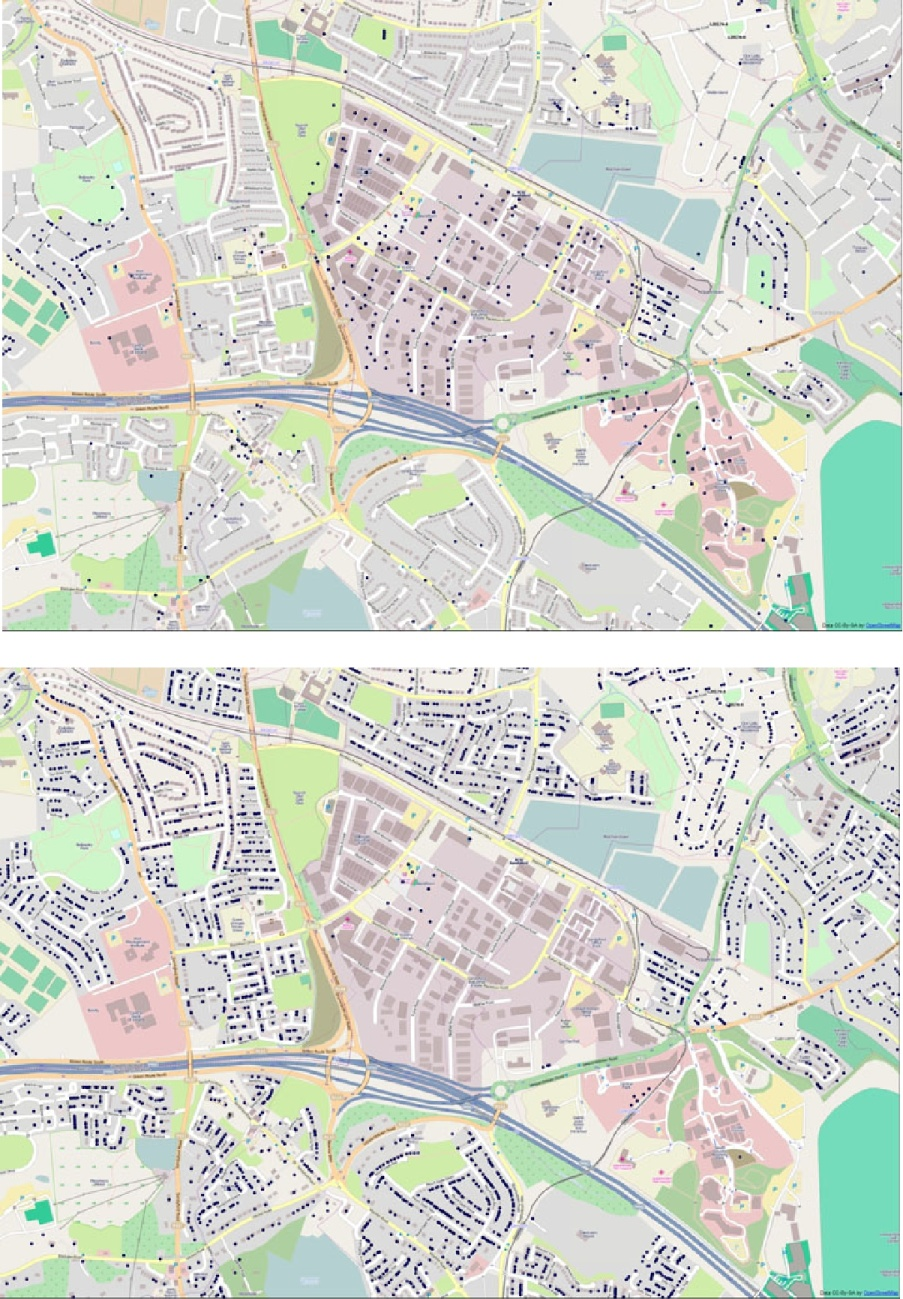
\includegraphics[width=0.99\textwidth, angle=0]{using/figures/dublin0.png}}%
{}
% ------------

% ------------
\createfigure%
{Hourly observed traffic volumes (dashed line) compared to the estimated traffic volumes produced by MATSim using the radiation model (green line) and nearest neighbor model (orange line).}%
{Hourly observed traffic volumes compared to the estimated traffic volumes}%
{\label{fig:dublin1}}%
{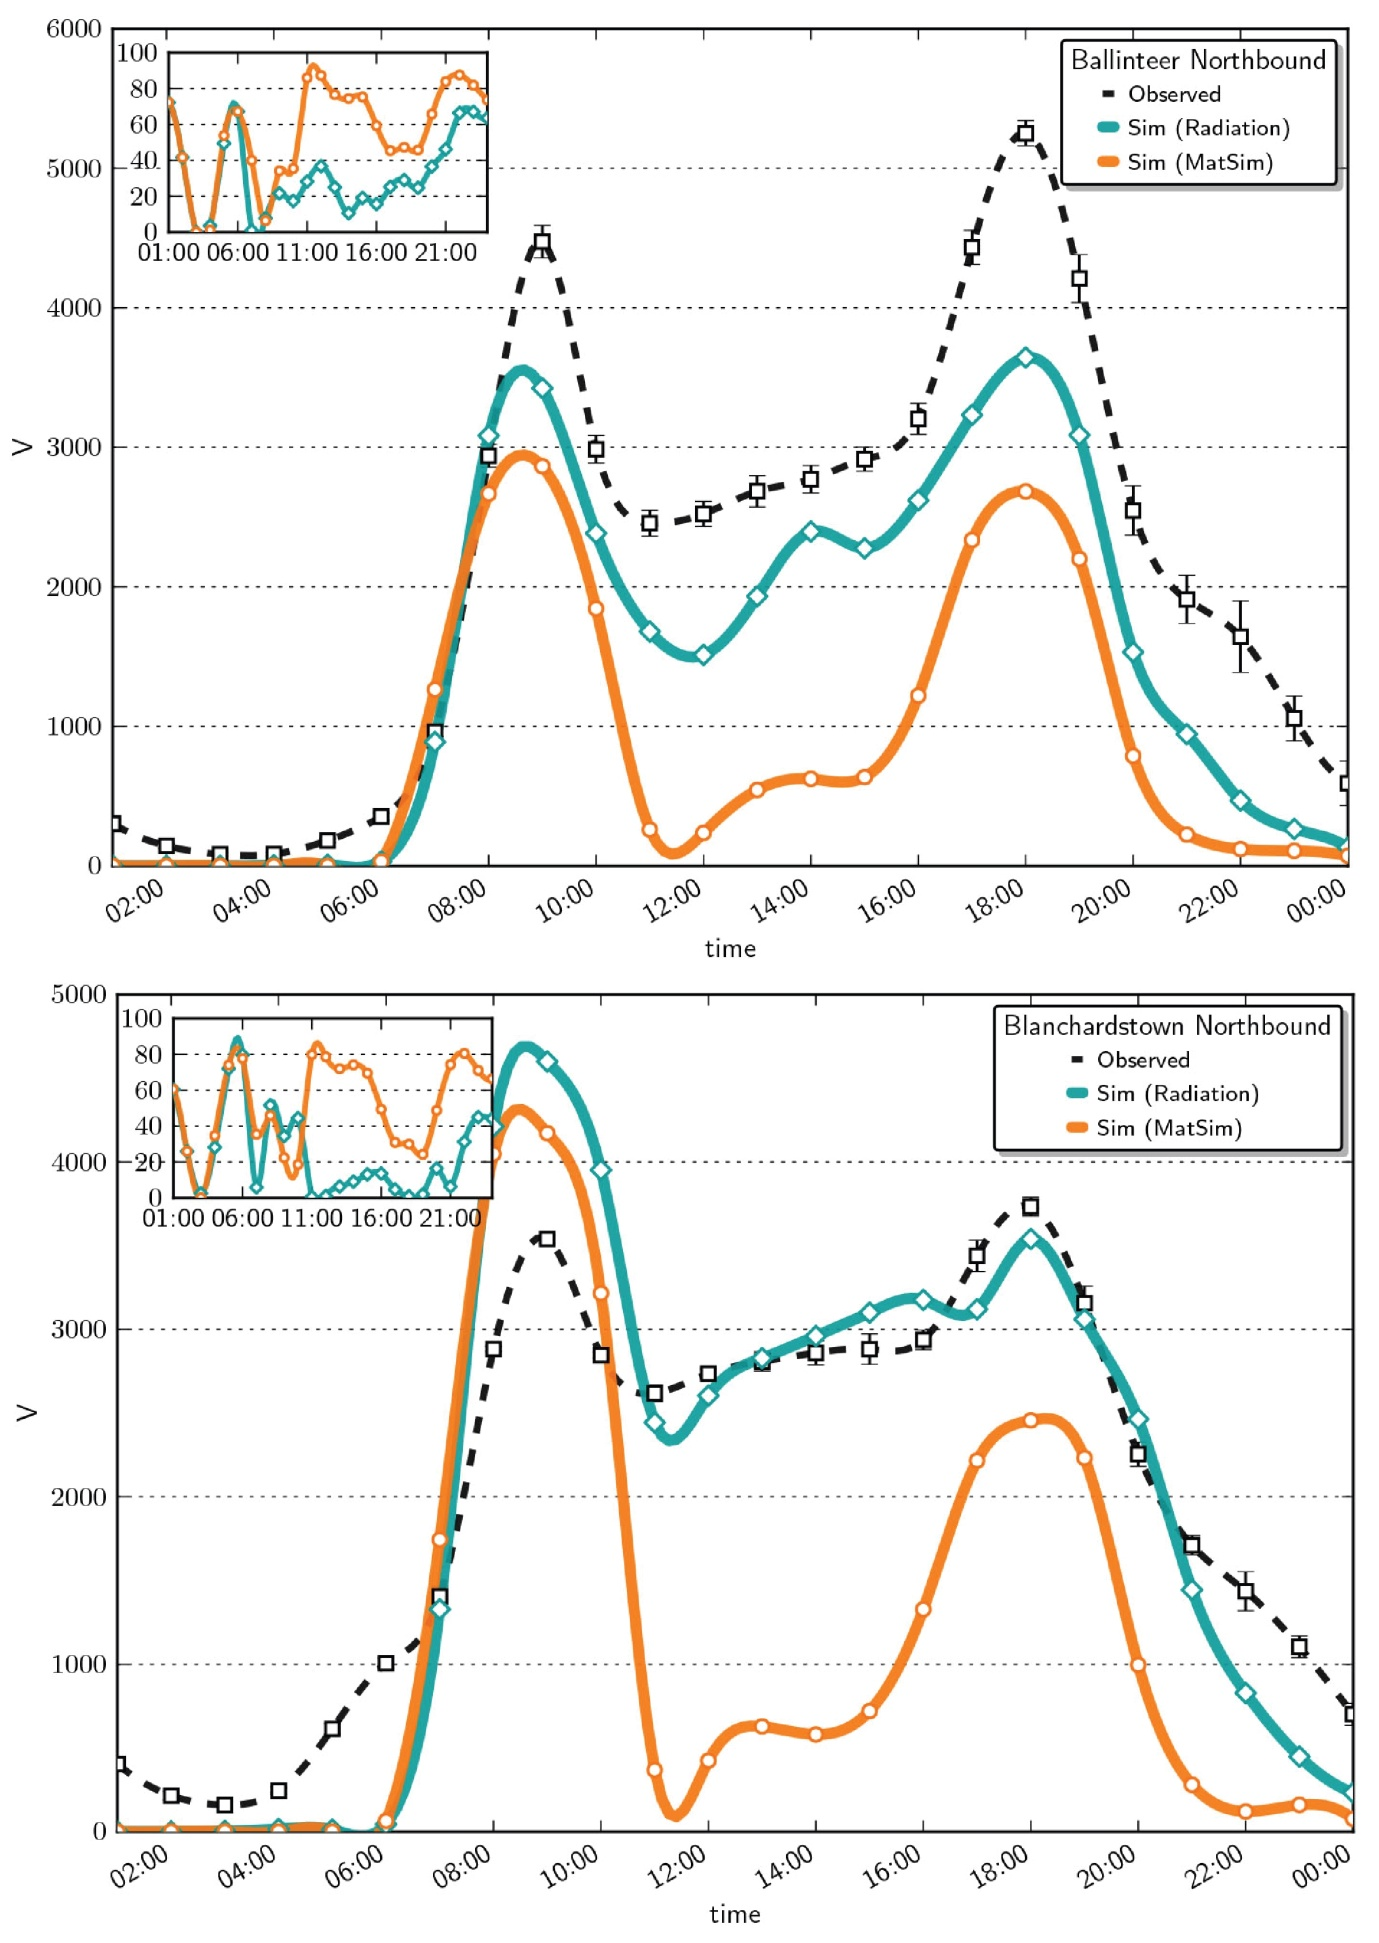
\includegraphics[width=0.99\textwidth, angle=0]{using/figures/dublin1.png}}%
{}
% ------------

% =======================================================================================





